
\documentclass{beamer}



\mode<presentation>
{
  \usetheme{Warsaw}
  % or ...

  \setbeamercovered{transparent}
  % or whatever (possibly just delete it)
}


\usepackage [english]{babel} 
% or whatever

\usepackage[utf8]{inputenc}
% or whatever

\usepackage{times}
\usepackage[T1]{fontenc}
% Or whatever. Note that the encoding and the font should match. If T1
% does not look nice, try deleting the line with the fontenc.


\title{IDE}

\subtitle
{Integrated Development Environment}

\author[Garçon, Chiron, Cassaing] % (optional, use only with lots of authors)
{B.~Garçon\inst{1} \and L.~Chiron\inst{2} \and M.~Cassaing\inst{3}}
% - Give the names in the same order as the appear in the paper.
% - Use the \inst{?} command only if the authors have different
%   affiliation.

\institute[ISIMA] % (optional, but mostly needed)
{
  \inst{1}%
  Étudiant de Prep'ISIMA
  \and
  \inst{2}%
  Étudiant de Prep'ISIMA
  \and
  \inst{3}%
  Étudiante de Prep'ISIMA}
% - Use the \inst command only if there are several affiliations.
% - Keep it simple, no one is interested in your street address.

\date[SGL 2013] % (optional, should be abbreviation of conference name)
{Soutenance du module de Génie Logiciel, 2013}
% - Either use conference name or its abbreviation.
% - Not really informative to the audience, more for people (including
%   yourself) who are reading the slides online

\subject{Theoretical Computer Science}
% This is only inserted into the PDF information catalog. Can be left
% out. 



% If you have a file called "university-logo-filename.xxx", where xxx
% is a graphic format that can be processed by latex or pdflatex,
% resp., then you can add a logo as follows:

\pgfdeclareimage[height=0.5cm]{university-logo}{../images/isima.png}
\logo{\pgfuseimage{university-logo}}




% If you wish to uncover everything in a step-wise fashion, uncomment
% the following command: 

%\beamerdefaultoverlayspecification{<+->}


\begin{document}

\begin{frame}
  \titlepage
\end{frame}

\begin{frame}{Outline}
  \tableofcontents
  % You might wish to add the option [pausesections]
\end{frame}


% Structuring a talk is a difficult task and the following structure
% may not be suitable. Here are some rules that apply for this
% solution: 

% - Exactly two or three sections (other than the summary).
% - At *most* three subsections per section.
% - Talk about 30s to 2min per frame. So there should be between about
%   15 and 30 frames, all told.

% - A conference audience is likely to know very little of what you
%   are going to talk about. So *simplify*!
% - In a 20min talk, getting the main ideas across is hard
%   enough. Leave out details, even if it means being less precise than
%   you think necessary.
% - If you omit details that are vital to the proof/implementation,
%   just say so once. Everybody will be happy with that.

\section{Qu'est-ce qu'un IDE ?}

\subsection{Historique}
\begin{frame}{Make Titles Informative.}
\end{frame}

\begin{frame}{Make Titles Informative.}
\end{frame}



\subsection{Les fonctionnalités}

\begin{frame}{Make Titles Informative. Use Uppercase Letters.}{Subtitles are optional.}
  % - A title should summarize the slide in an understandable fashion
  %   for anyone how does not follow everything on the slide itself.

  \begin{itemize}
  \item
    Use \texttt{itemize} a lot.
  \item
    Use very short sentences or short phrases.
  \end{itemize}
\end{frame}

\begin{frame}{Make Titles Informative.}

  You can create overlays\dots
  \begin{itemize}
  \item using the \texttt{pause} command:
    \begin{itemize}
    \item
      First item.
      \pause
    \item    
      Second item.
    \end{itemize}
  \item
    using overlay specifications:
    \begin{itemize}
    \item<3->
      First item.
    \item<4->
      Second item.
    \end{itemize}
  \item
    using the general \texttt{uncover} command:
    \begin{itemize}
      \uncover<5->{\item
        First item.}
      \uncover<6->{\item
        Second item.}
    \end{itemize}
  \end{itemize}
\end{frame}



\section{Code::Blocks : un IDE pour vous}

\subsection{Création d'un projet assisté}

\begin{frame}{Make Titles Informative.}
\begin{figure}
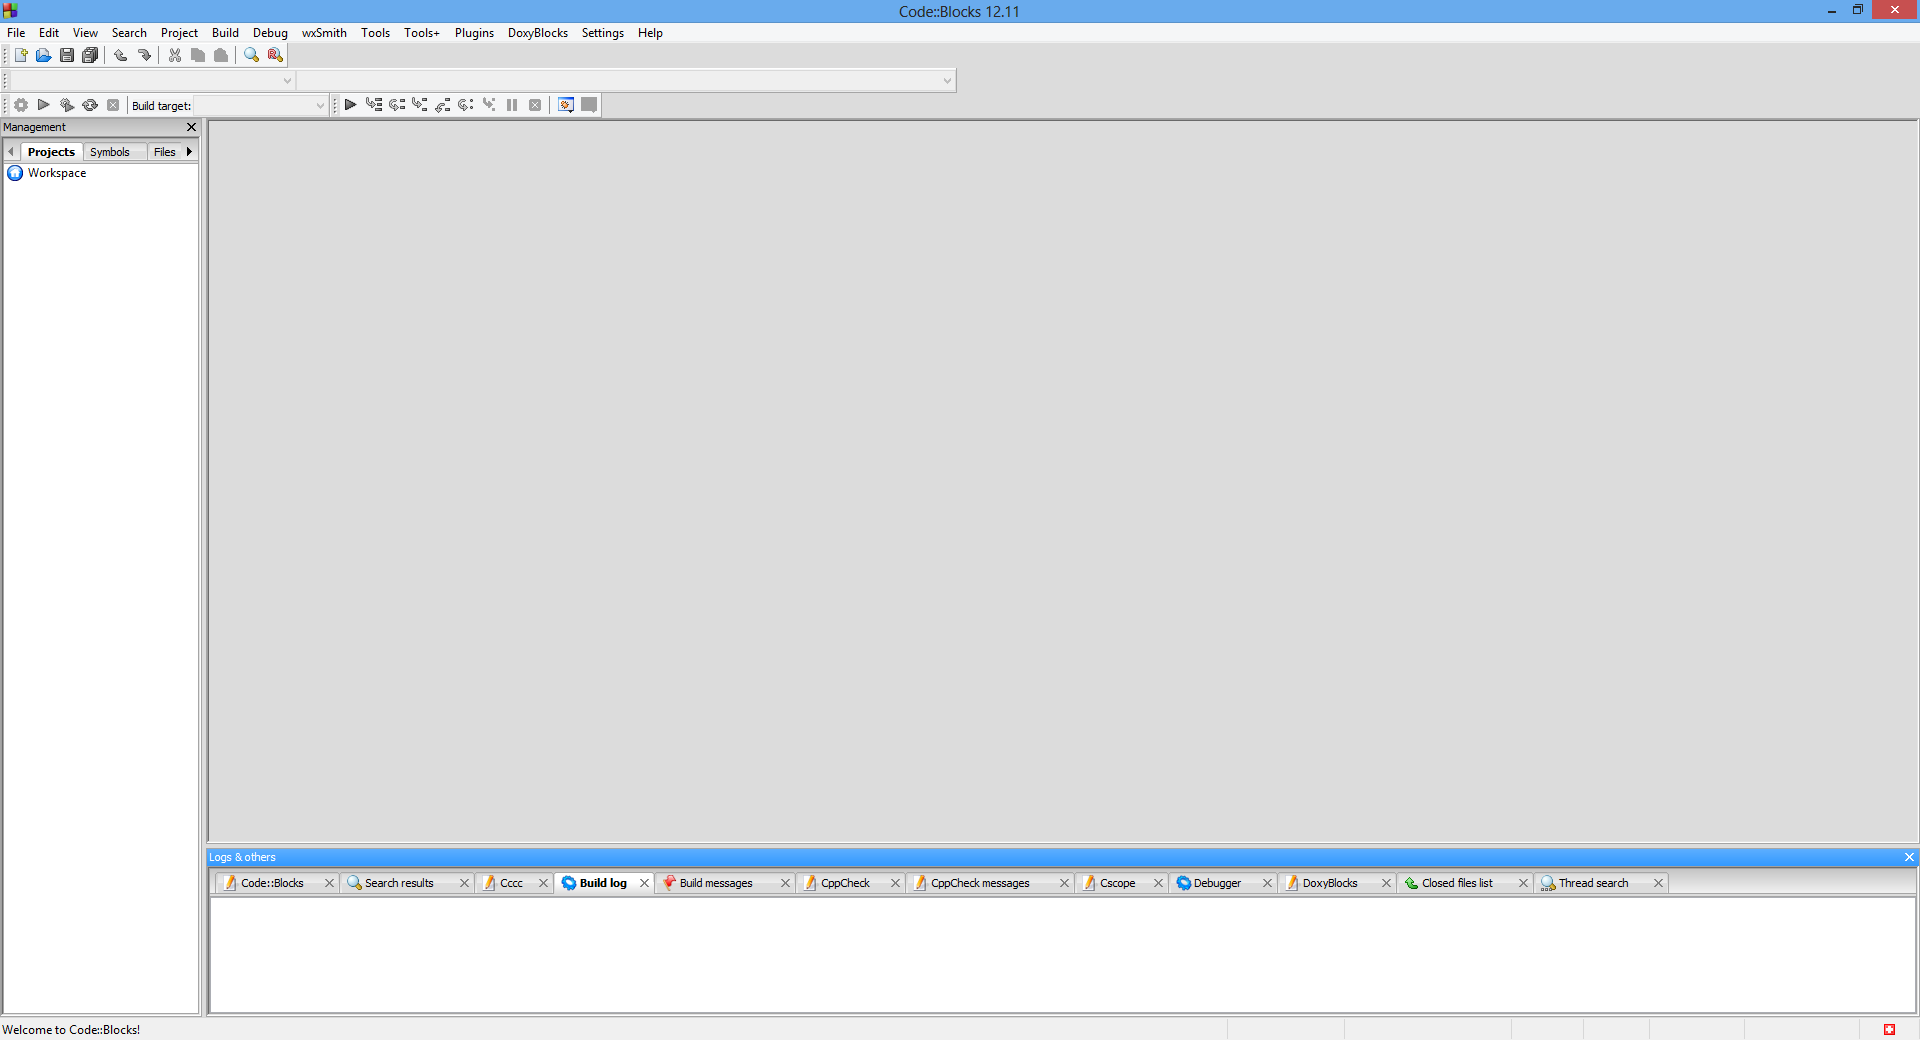
\includegraphics[scale=0.3]{../images/cb01.png}
\caption{Code::Blocks}				
\label{cb01}				
\end{figure}
\end{frame}

\begin{frame}{Make Titles Informative.}
\begin{figure}
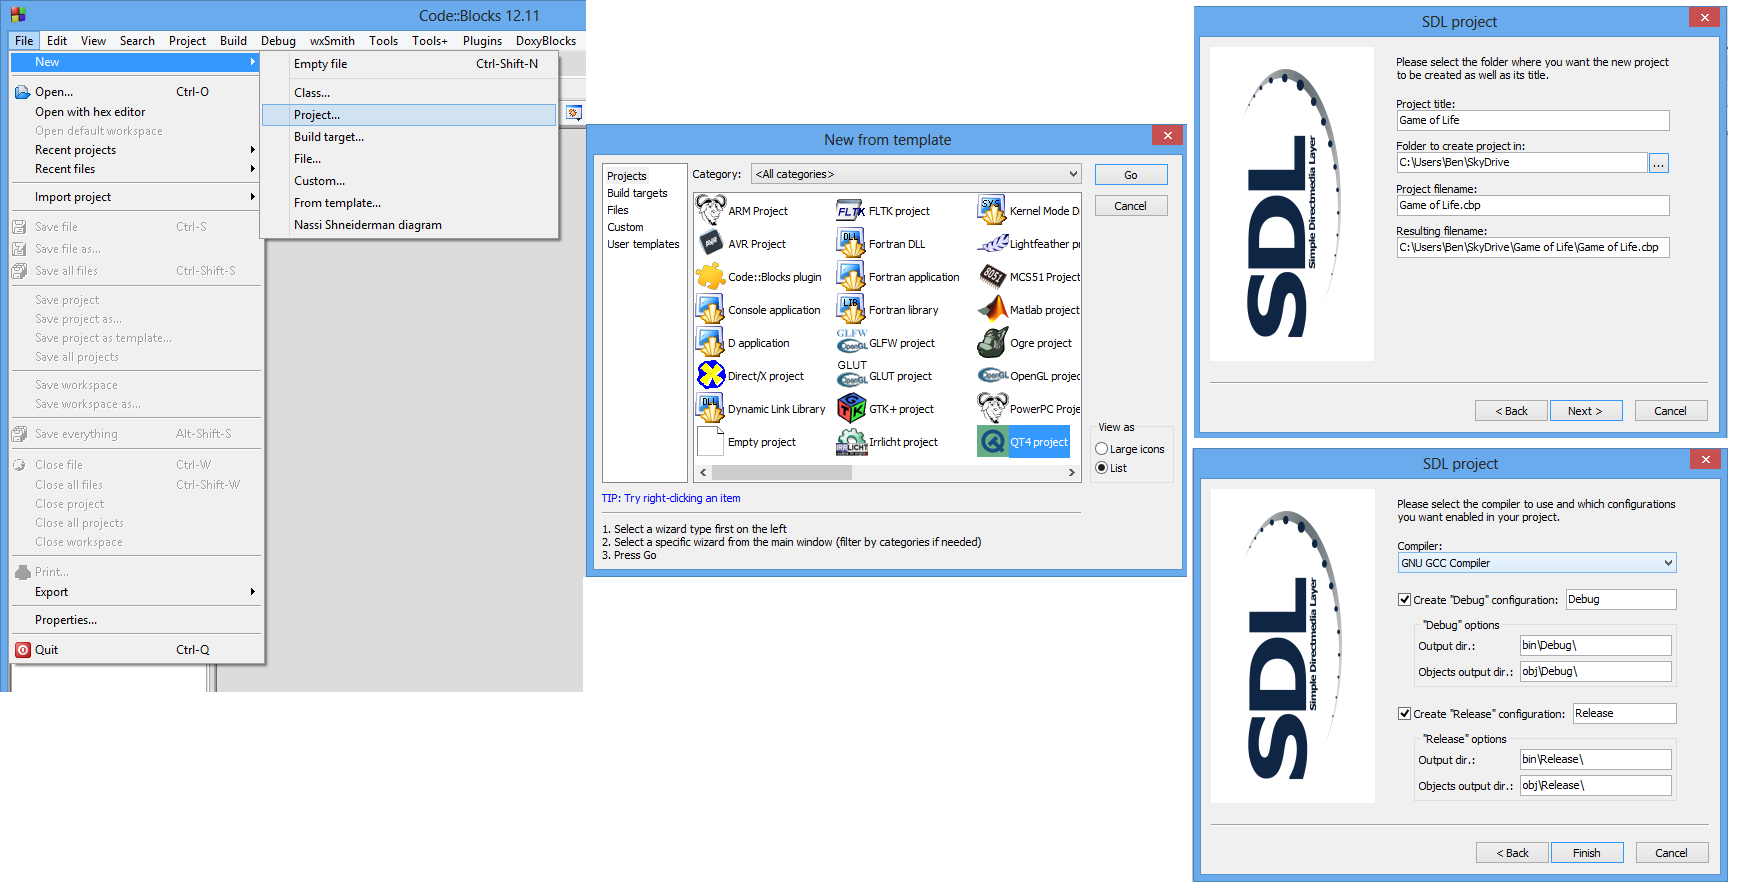
\includegraphics[scale=0.35]{../images/cb02.png}
\caption{Configuration du nouveau projet}				
\label{cb02}				
\end{figure}
\end{frame}

\begin{frame}{Make Titles Informative.}
\begin{figure}
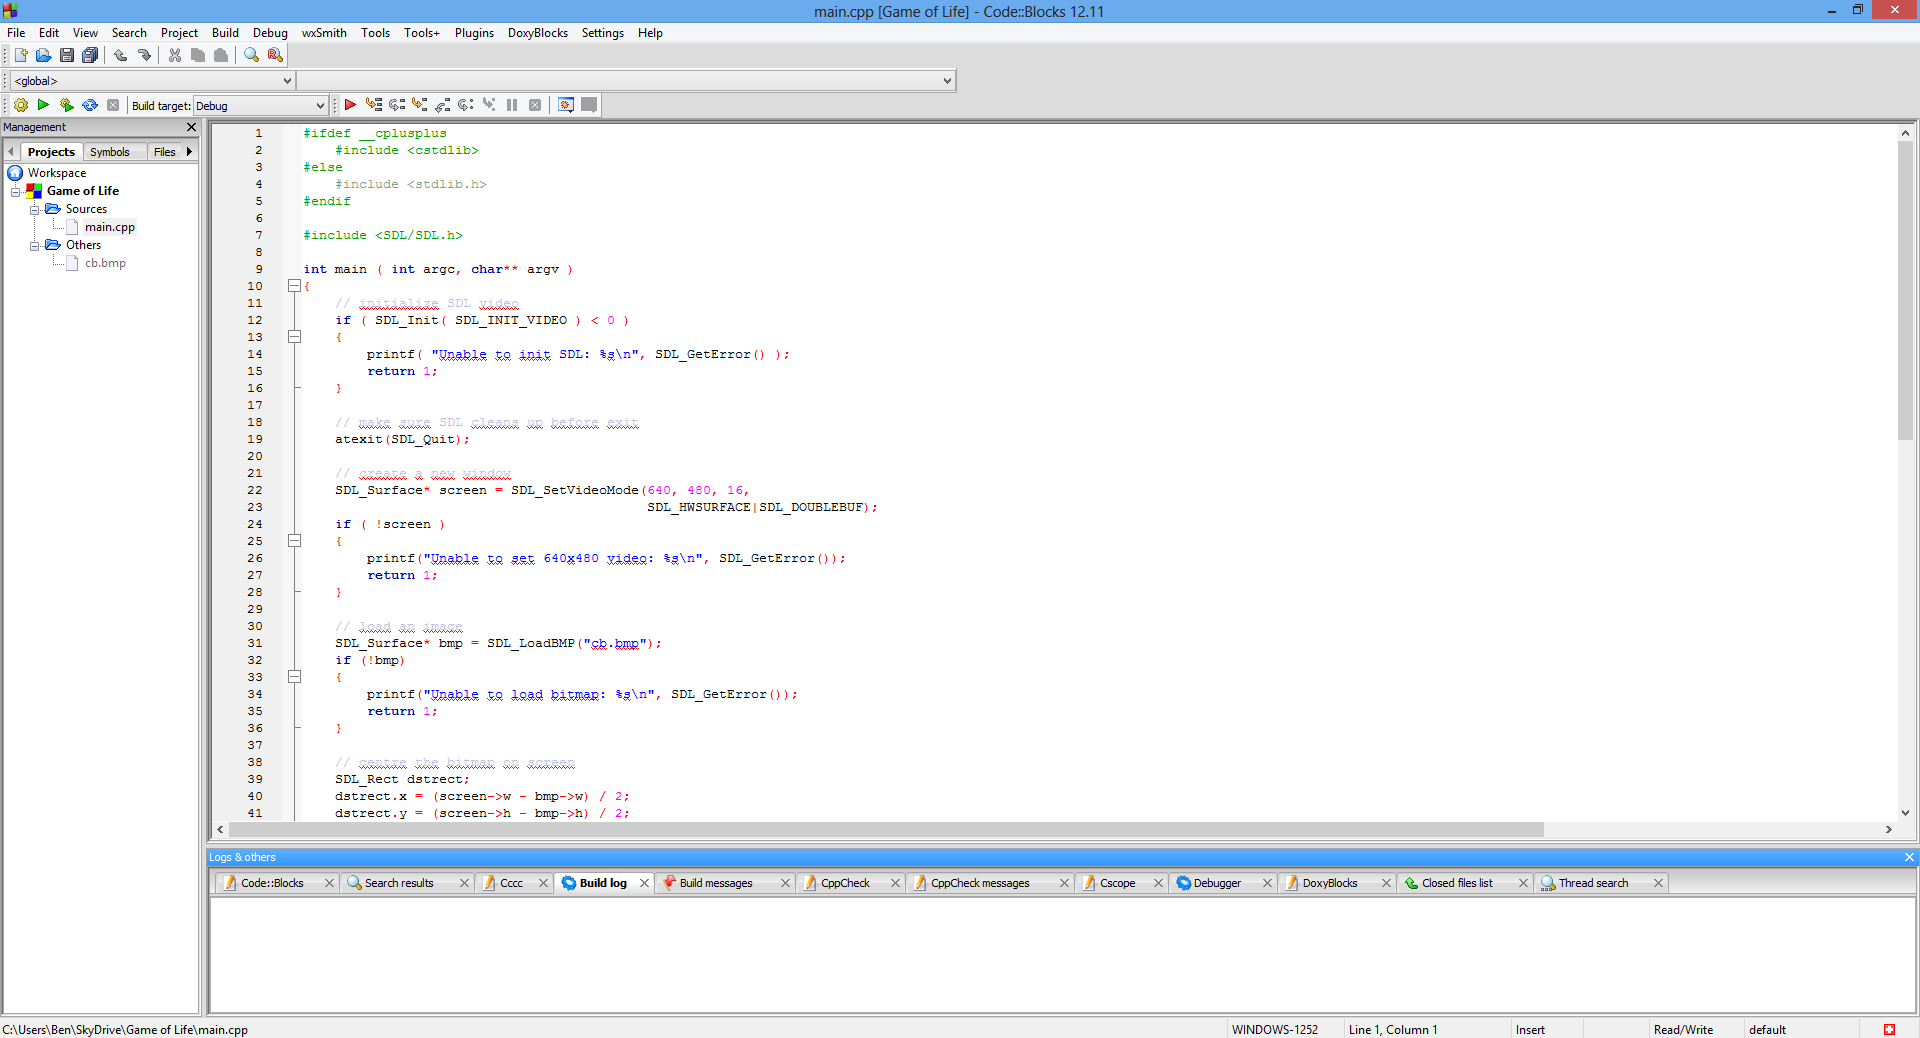
\includegraphics[scale=0.35]{../images/cb03.png}
\caption{Code par défaut clé en main}				
\label{cb03}				
\end{figure}
\end{frame}


\subsection{Programmation sous Code::Blocks}

\begin{frame}{Make Titles Informative.}
\begin{figure}
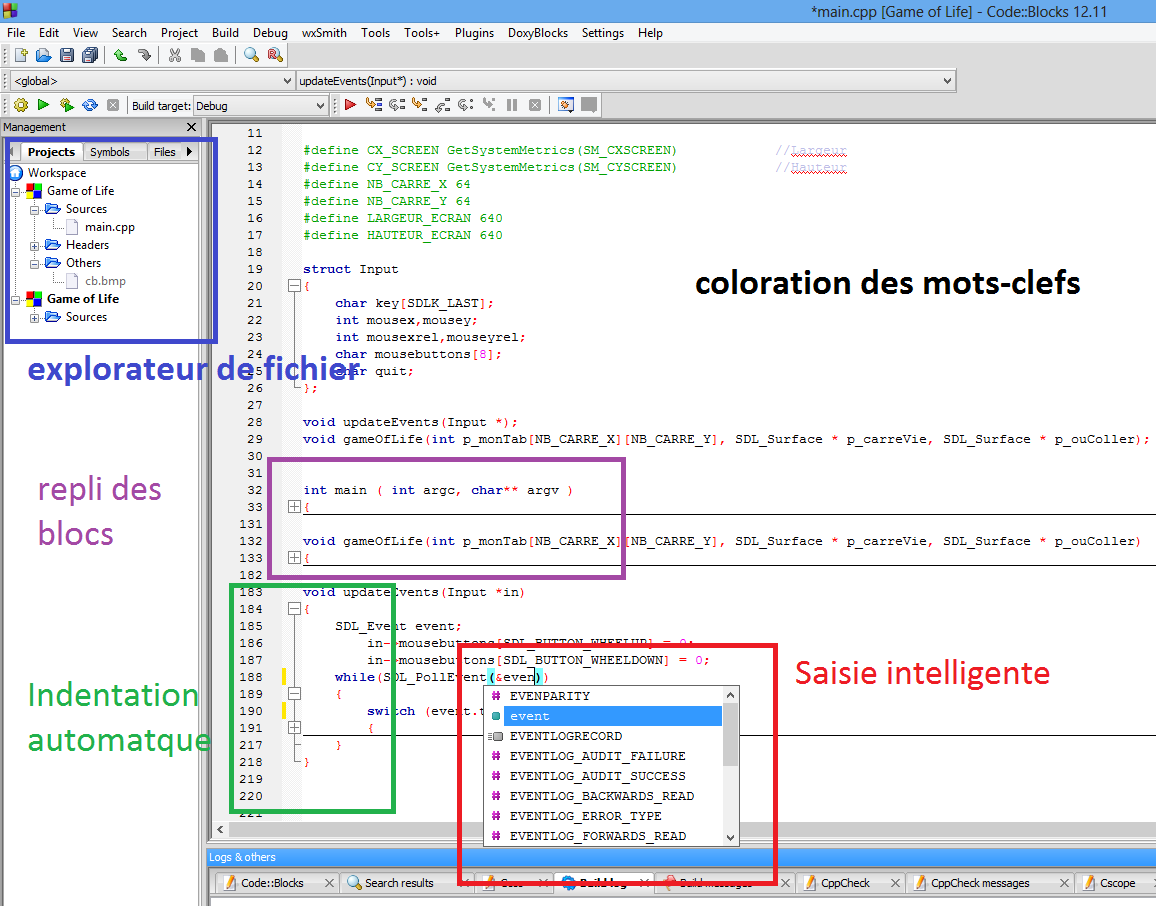
\includegraphics[scale=0.55]{../images/cb04.png}
\caption{Fonctionnalités intéressantes de l'éditeur de texte}				
\label{cb04}				
\end{figure}
\end{frame}

\begin{frame}{Make Titles Informative.}
\begin{figure}
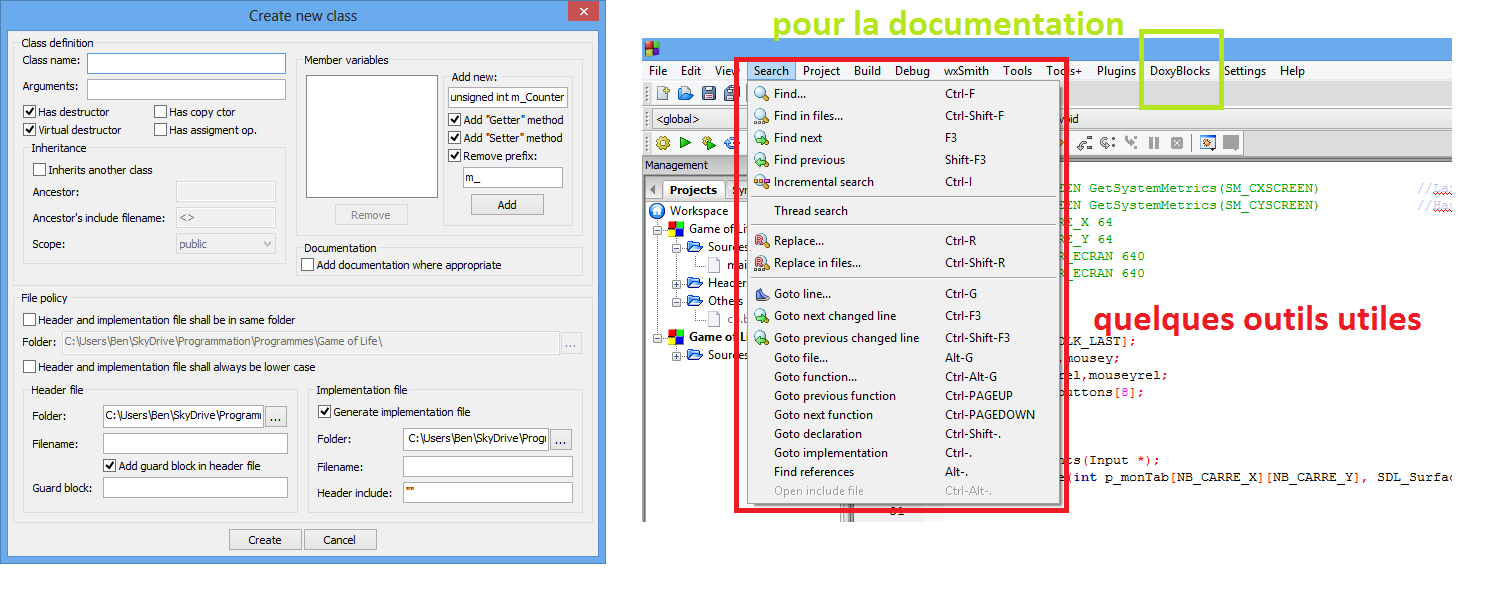
\includegraphics[scale=0.45]{../images/cb05.png}
\caption{Quelques outils pratiques}				
\label{cb05}				
\end{figure}
\end{frame}

\begin{frame}{Make Titles Informative.}
\end{frame}


\subsection{Finalisation du programme avec Code::Blocks}

\begin{frame}{Make Titles Informative.}
\begin{figure}
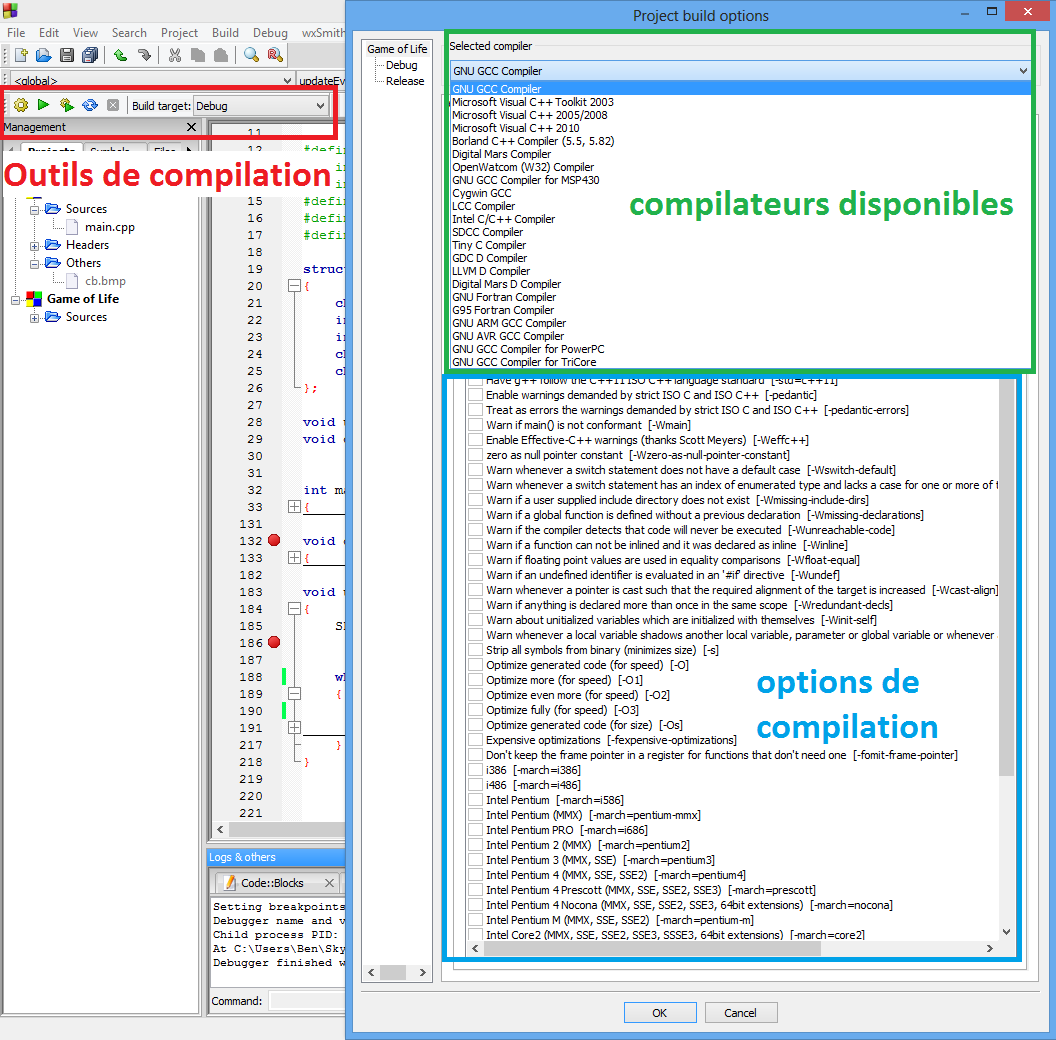
\includegraphics[scale=0.6]{../images/cb06.png}
\caption{La compilation}				
\label{cb06}				
\end{figure}
\end{frame}

\begin{frame}{Make Titles Informative.}
\begin{figure}
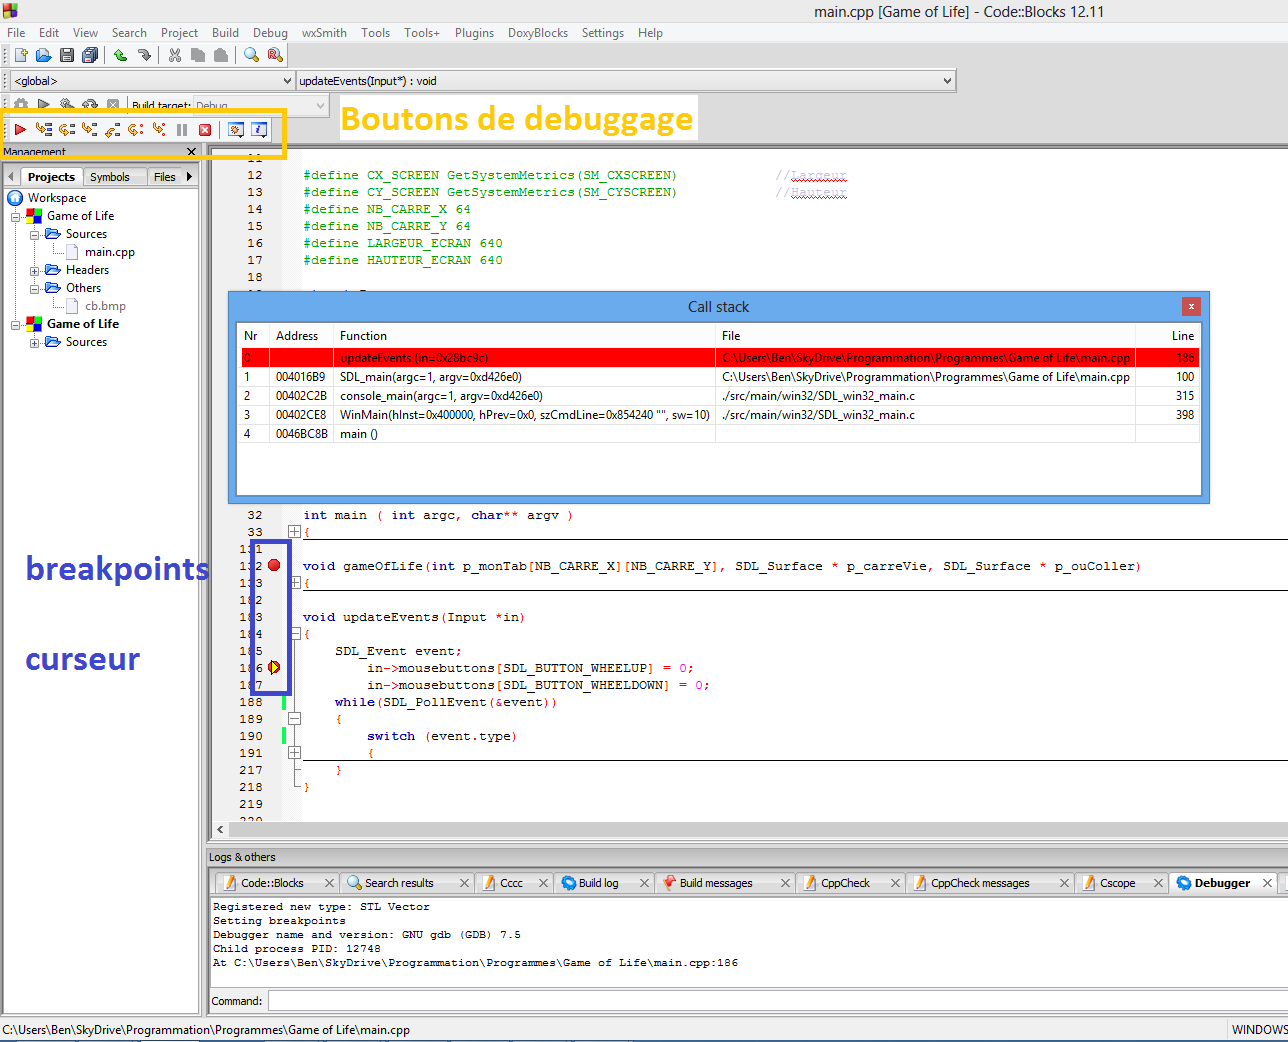
\includegraphics[scale=0.5]{../images/cb07.png}
\caption{Le débuggage}				
\label{cb07}				
\end{figure}
\end{frame}

\begin{frame}{Make Titles Informative.}
\end{frame}


\section*{Bilan}

\begin{frame}{Bilan}

  % Keep the summary *very short*.
  \begin{itemize}
  \item
    The \alert{first main message} of your talk in one or two lines.
  \item
    The \alert{second main message} of your talk in one or two lines.
  \item
    Perhaps a \alert{third message}, but not more than that.
  \end{itemize}
  
  % The following outlook is optional.
  \vskip0pt plus.5fill
  \begin{itemize}
  \item
    Outlook
    \begin{itemize}
    \item
      Something you haven't solved.
    \item
      Something else you haven't solved.
    \end{itemize}
  \end{itemize}
\end{frame}



% All of the following is optional and typically not needed. 
\appendix
\section<presentation>*{\appendixname}
\subsection<presentation>*{Pour plus de programmation ...}

\begin{frame}[allowframebreaks]
  \frametitle<presentation>{Pour plus de programmation ...}
    
  \begin{thebibliography}{10}
    
  \beamertemplateonlinebibitems
  % Start with overview books.

  \bibitem{cle}
    Eclipse
    \newblock {\em Handbook of Everything}.
    \newblock Some Press, 1990.
 
    
  \beamertemplateonlinebibitems
  % Followed by interesting articles. Keep the list short. 

  \bibitem{Someone2000}
    NetBeans
    \newblock On this and that.
    \newblock {\em Journal of This and That}, 2(1):50--100,
    2000.
  \end{thebibliography}
\end{frame}

\end{document}


